\documentclass{article}
\usepackage[utf8]{inputenc}
\usepackage{amsfonts}\usepackage{amssymb}\usepackage{amsmath}
\usepackage[top=2cm,left=1cm,right=1cm]{geometry}\usepackage{tikz}
\usepackage{gensymb}\usepackage{ragged2e}\usepackage{blindtext}\usepackage{polynom} \usepackage{graphicx}
\begin{document}
\begin{center}
     MAT110 ASSIGNMENT 2 [SET-03]\\[6pt]
    NAME: ANIKA ISLAM \\[6pt]
    ID:21101298 \\[6pt]
    SECTION:08
\end{center}
\newpage 
\begin{figure}[htbp!]
    \centering
    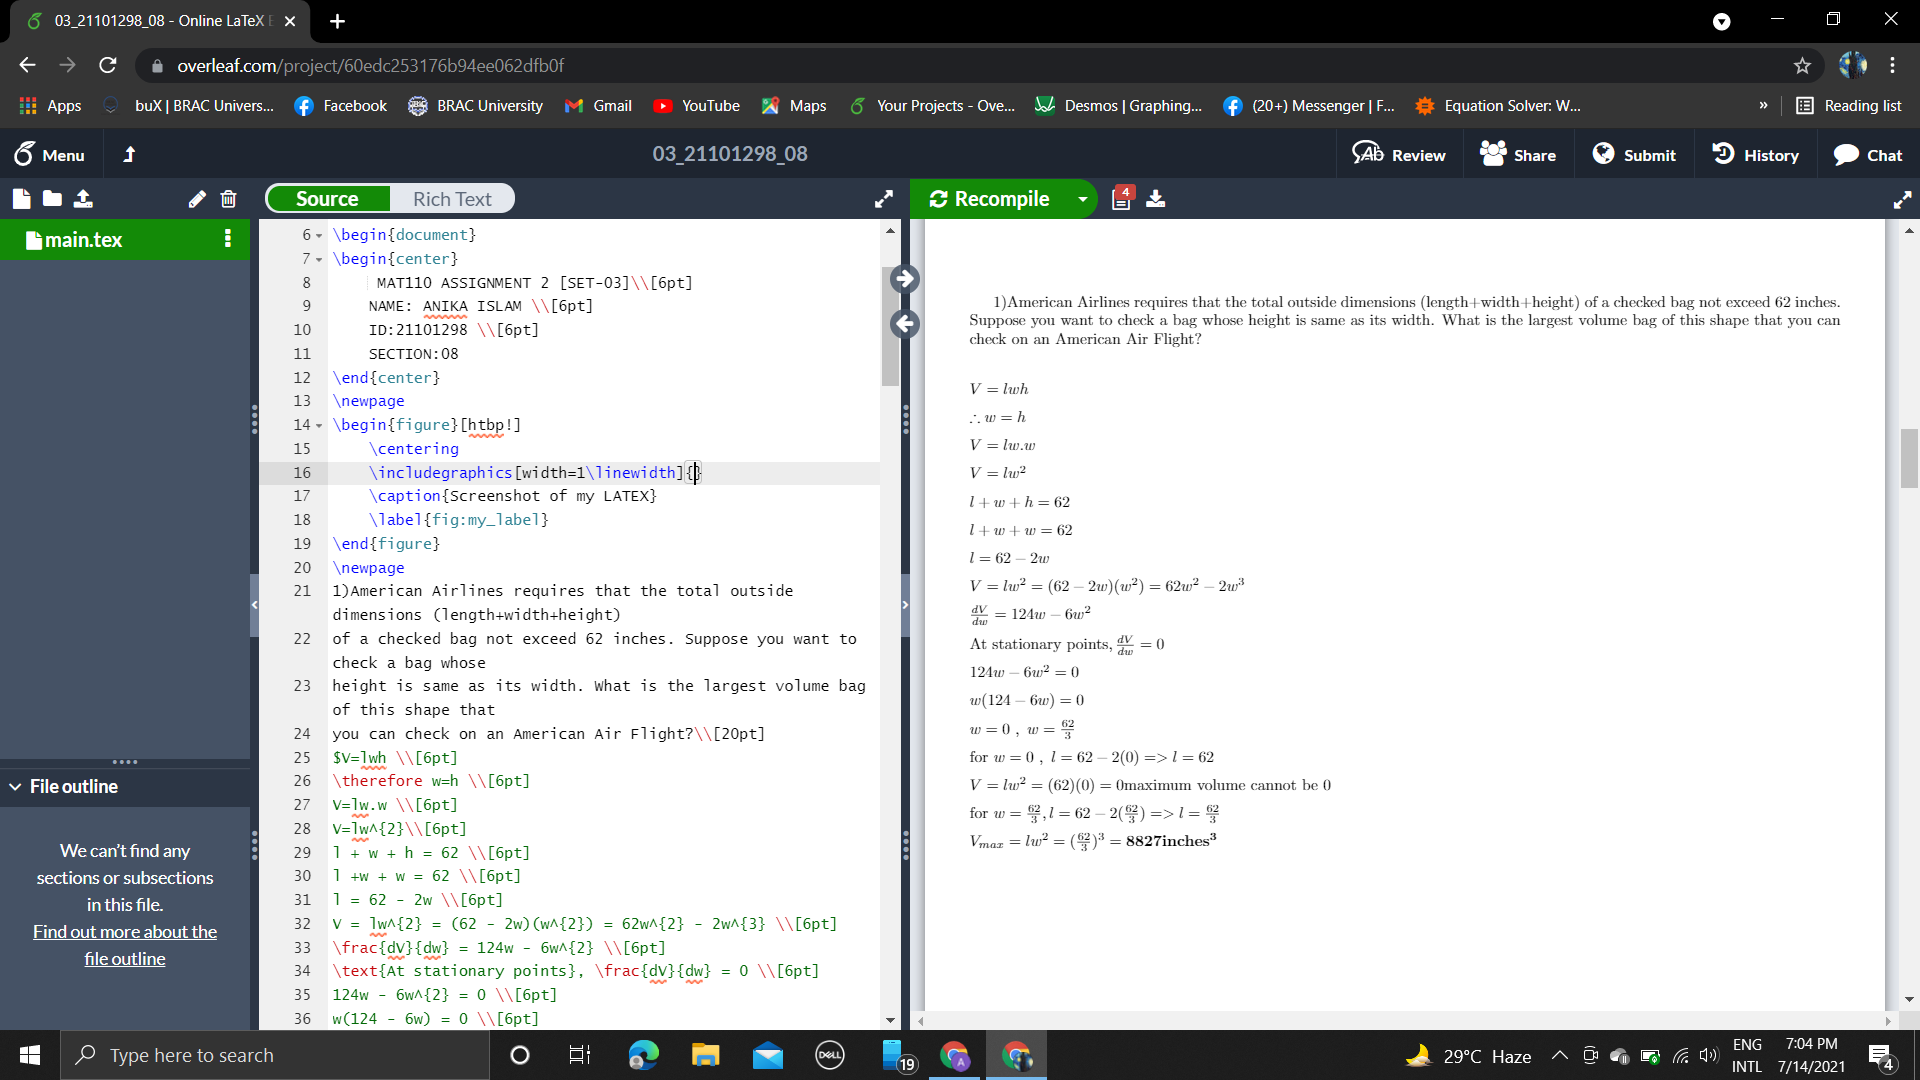
\includegraphics[width=1\linewidth]{SET 3.png}
    \caption{Screenshot of my LATEX}
    \label{fig:my_label}
\end{figure}
\newpage 
1)American Airlines requires that the total outside dimensions (length+width+height)
of a checked bag not exceed 62 inches. Suppose you want to check a bag whose
height is same as its width. What is the largest volume bag of this shape that
you can check on an American Air Flight?\\[20pt]
$V=lwh \\[6pt]
\therefore w=h \\[6pt]
V=lw.w \\[6pt]
V=lw^{2}\\[6pt]
l + w + h = 62 \\[6pt]
l +w + w = 62 \\[6pt]
l = 62 - 2w \\[6pt]
V = lw^{2} = (62 - 2w)(w^{2}) = 62w^{2} - 2w^{3} \\[6pt]
\frac{dV}{dw} = 124w - 6w^{2} \\[6pt]
\text{At stationary points}, \frac{dV}{dw} = 0 \\[6pt]
124w - 6w^{2} = 0 \\[6pt]
w(124 - 6w) = 0 \\[6pt]
w = 0  \ , \   w = \frac{62}{3} \\[6pt]$
$ \text{for} \  w = 0 \ , \ l = 62 - 2(0) => l =62 \\[6pt]
V = lw^{2} = (62)(0) = 0  \ \text{(maximum volume cannot be 0)}\\[6pt]
\text{for} \  w = \frac{62}{3} , l = 62 - 2(\frac{62}{3}) => l = \frac{62}{3} \\[6pt]
V_{max} = lw^{2} = (\frac{62}{3})^{3} = \mathbf{8827 inches^{3}}$ \\[20pt]

\newpage 
2)With the help of Leibniz’s theorem find $y_5$ of $y = (x^{3} + 2x^{2})e^{2x}$\\[20pt]
$y_5$ of $y = (x^{3}+ 2x^{2})e^{2x} \\[6pt]
1st \rightarrow 5^{0} = 1 \\[6pt]
2nd \rightarrow 5^{1} = 5 \\[6pt]
3rd \rightarrow \frac{5(5-1)}{2!} = 10 \\[6pt]
4th \rightarrow \frac{5(5-1)(5-2)}{3!} = 10 \\[6pt]
5th \rightarrow \frac{5(5-1)(5-2)(5-3)}{4!} = 5\\[6pt]
6th \rightarrow \frac{5(5-1)(5-2)(5-3)(5-4)}{5!} = 1 \\[6pt]$
\begin{table}[htbp!]
    \centering
    \begin{tabular}{c|c}
        $u=x^{3} + 2x^{2}$ & $v=e^{2x}$ \\
        $u'=3x^{2} + 4x$ & $v'=2e^{2x}$ \\
        $u''=6x + 4$ & $v''=4e^{2x}$ \\
        $u'''=6 $ & $v'''=8e^{2x}$ \\
        $u^{4}=0$ & $v^{4}=16e^{2x}$ \\
        $u^{5}=0$ & $v^{5}=32e^{2x}$ \\
    \end{tabular}
\end{table}\\[6pt]
$y_{5}=uv^{5} + 5u'v^{4} + 10u''v''' + 10u'''v'' + 5u^{4}v' + u^{5}v \\[6pt] 
y_{5} = (x^{3} + 2x^{2})(32e^{2x}) + 5(3x^{2} + 4x)(16e^{2x}) + 10(6x + 4)(8e^{2x}) + 10(6)(4e^{2x}) + 5(0)(2e^{2x}) + 1(0)(e^{2x}) \\[6pt]
y_{5} = (x^{3} + 2x^{2})(32e^{2x}) + 5(3x^{2} + 4x)(16e^{2x}) + 10(6x + 4)(8e^{2x}) + 10(6)(4e^{2x})\\[6pt]
y_{5} = 4e^{2x}(8x^{3} + 16x^{2} + 60x^{2} + 80x + 120x + 80 +60 ) \\[6pt]
\mathbf{y_{5} = 4e^{2x}(8x^{3} + 76x^{2} + 200x + 140)}$\\[20pt]

\newpage 
3)Let p denote the number of paramecia in a nutrient solution t days after the
start of an experiment, and assume that p is defined implicitly as a function
of t by the equation $0 = \ln p + 0.83 - \ln (2.3 - 0.0046p) - 2.3t$ Use implicit
differentiation to show that the rate of change of p with respect to t satisfies
the equation:
$\frac{dp}{dt} = 0.0046p(500 -  p).$ \\[20pt]
$ \ln p + 0.83 - \ln (2.3 - 0.0046p) - 2.3t = 0 \\[6pt]
=>\frac{1}{p} \frac{dp}{dt} + 0 +\frac{-0.0046}{2.3 - 0.0046p} \frac{dp}{dt} - 2.3 = 0\\[6pt]
=> \frac{dp}{dt} (\frac{1}{p} + \frac{-0.0046}{2.3 - 0.0046p}) = 2.3 \\[6pt]
=> \frac{dp}{dt} (\frac{2.3 - 0.0046p + 0,0046p}{(2.3 - 0.0046p)p}) = 2.3 \\[6pt]
=> \frac{dp}{dt} = (2.3 - 0.0046p)p \\[6pt]
=> \mathbf{\frac{dp}{dt} = 0.0046p(500 - p)} \\[20pt]$

\newpage 
4)Use logarithm function to find out the first derivative of
$y =\frac{(x^{2} - 8)^{\frac{1}{3}}\sqrt{x^{3} + 1}}{x^{6} -  7x + 5}$\\[20pt]
$y =\frac{(x^{2} - 8)^{\frac{1}{3}}\sqrt{x^{3} + 1}}{x^{6} -  7x + 5} \\[6pt]
=> \ln y = \ln \frac{(x^{2} - 8)^{\frac{1}{3}}\sqrt{x^{3} + 1}}{x^{6} -  7x + 5} \\[6pt]
=> \ln y = \ln (x^{2} - 8)^{\frac{1}{3}} + \ln (\sqrt{x^{3} + 1}) - \ln (x^{6} -7x +5)\\[6pt]
=> \frac{1}{y} \frac{dy}{dx} = \frac{\frac{1}{3}(2x)(x^{2} - 8)^{-\frac{2}{3}}}{(x^{2} - 8)^{\frac{1}{3}}} + \frac{\frac{1}{2}(3x^{2})(x^{3} +1 )^{-\frac{1}{2}}}{(x^{3} + 1 )^{\frac{1}{2}}} - \frac{6x^{5} -7}{x^{6} - 7x +5} \\[6pt]
=> \frac{1}{y} \frac{dy}{dx} = \frac{2x}{3(x^{2} - 8)} + \frac{3x^{2}}{2(x^{3} + 1 )} - \frac{6x^{5} -7}{x^{6} - 7x +5} \\[6pt]
=> \frac{1}{y} \frac{dy}{dx} = \frac{2x(x^{2} - 8)^{-\frac{2}{3}}}{3(x^{2} - 8)^{\frac{1}{3}}} + \frac{3x^{2}(x^{3} +1 )^{-\frac{1}{2}}}{2(x^{3} + 1 )^{\frac{1}{2}}} - \frac{6x^{5} -7}{x^{6} - 7x +5} \\[6pt]
=> \frac{1}{y}\frac{dy}{dx} = \frac{2x}{3(x^{2} - 8)} + \frac{3x^{2}}{2(x^{3} + 1 )} - \frac{6x^{5} -7}{x^{6} - 7x +5} \\[6pt]
=> \frac{dy}{dx} = y \left[\frac{2x}{3(x^{2} - 8)} + \frac{3x^{2}}{(2(x^{3} + 1 )} - \frac{6x^{5} -7}{x^{6} - 7x +5} \right] \\[6pt]
=> \mathbf{\frac{dy}{dx} = \left[\frac{(x^{2} - 8)^{\frac{1}{3}}\sqrt{x^{3} + 1}}{x^{6} -  7x + 5}\right] \left[\frac{2x}{3(x^{2} - 8)} + \frac{3x^{2}}{2(x^{3} + 1 )} - \frac{6x^{5} -7}{x^{6} - 7x +5} \right]}$ \\[20pt]

\newpage 
5)Let $f(x) = (-\cos x + \sin x)$ over the interval $[-\pi, \pi]$. Use the first and second
derivatives of f to determine where f is increasing, decreasing, concave up,
and concave down. Locate all inflection points,if they exist.[20pt]
$f(x) = -\cos x + \sin x\\[6pt]
f'(x) = \sin x + \cos x \\[6pt]
\text{At stationary point} \ , \ f'(x) = 0 \\[6pt]
=> 0 = \sin x + \cos x \\[6pt]
=> \tan x = -1 \\[6pt]
=> x = -\frac{\pi}{4} \ , \  x = \frac{3\pi}{4} \\[6pt]$
\begin{table}[htbp!]
    \centering
    \begin{tabular}{c|c|c|c}
        Intervals & $f'(x)$ & Sign & Conclusion \\[6pt]
         $(-\pi,-\frac{\pi}{4})$ & $\sin x  + \cos x$ & -ve & decreasing \\[6pt]
         $(-\frac{\pi}{4},\frac{3\pi}{4})$ & $\sin x  + \cos x$ & +ve & increasing \\[6pt]
         $(\frac{3\pi}{4},\pi)$ & $\sin x  + \cos x$ & +ve & increasing
    \end{tabular}
\end{table} \\[6pt]
$ \textbf{for} \  \mathbf{(-\pi,-\frac{\pi}{4}) \ ,f'(x)>0 \ ,\   f(x)} \  \textbf{is decreasing} \\[6pt]
\textbf{for} \ \mathbf{(-\frac{\pi}{4},\pi) \ , \ f'(x)<0 \ ,\  f(x)} \  \textbf{is increasing} \\[10pt]
f''(x) = \cos x - \sin x \\[6pt]
 f''(x) = 0 \\[6pt]
=> 0 = \cos x - \sin x\\[6pt]
=> \tan x = 1 \\[6pt]
x = \frac{\pi}{4} \\[6pt]$
\begin{table}[htbp!]
    \centering
    \begin{tabular}{c|c|c|c}
        Intervals & $f''(x)$ & Sign & Conclusion \\[6pt]
         $(-\pi,\frac{\pi}{4})$ & $\cos x  - \sin x$ & +ve & concave up  \\[6pt]
         $(\frac{\pi}{4},\pi)$ & $\cos x  - \sin x$ & -ve & concave down \\[6pt]
    \end{tabular}
\end{table} \\[6pt]
$ \textbf{for} \ \mathbf{(-\pi,\frac{\pi}{4}) \ , \ f''(x)>0 \ , \ f(x)} \  \textbf{is concave up} \\[6pt]
\textbf{for} \ \mathbf{(\frac{\pi}{4},\pi) \ , \ f''(x)<0 \ , \ f(x)} \ \textbf{is concave down} \\[6pt]
 \mathbf{ x = \frac{\pi}{4} }\  \textbf{is the inflection point.}\\[20pt]$

\newpage 
6)Find the relative extrema of $f(x) =\frac{x + 3}{x - 2}$\\[20pt]
$f(x) =\frac{x + 3}{x - 2}\\[6pt]
=> f'(x) = \frac{(x-2)\frac{d}{dx}(x + 3 ) - (x + 3)\frac{d}{dx}(x - 2)}{(x-2)^{2}}\\[6pt]
=> f'(x) = \frac{(x-2) - (x + 3)}{(x-2)^{2}}\\[6pt]
=> f'(x) = \frac{-5}{(x-2)^{2}}\\[6pt]
\text{At stationary points} \ , \ f'(x) = 0 \\[6pt]
=> \frac{-5}{(x-2)^{2}} = 0 \\[6pt]
=> -5 = 0 \\[6pt]
\textbf{Since, there is no value of x at the stationary point,hence no relative extrema exists}.\\[2pt]$
\end{document}
